\chapter*{Introduction}
\label{Introduction}

\section*{The decline of global biological diversity : state of the world}
\label{intro:facts}
% Setting the stage : global decline
Nature has been deterioting for the past centuries, and much has already been lost \citep{ipbes_2022_6417333}. Across all the scales of analysis, the state of nature is undoubtly critical. The structural conditions of ecosystems (e.g. different species that cause different structural phenomena and lead ecosystems to provide various resources, including wildlife habitat, carbon sequestration etc), the compositions (e.g. species richness\footnote{ Species richness measures the \textit{number of species} in a given period and location}) of ecological communities and populations (e.g. species abundance\footnote{ Species abundance measures the \textit{population of species} in a given period and location}) of species have experienced dramatic changes. 
% 5 lines for each
Ecosystem structure forms the basis of natural and social-ecological processes: their disruption have far reaching consequences. Overall, only 13\% of oceans and 23\% of land remains sufficiently unimpacted by humanity to be classified as \textit{wilderness} \citep{jones_2018_location, watson_2016_catastrophic}. While deforestation has slowed since the 1990s, \textit{vegetation biomass} (including trees) has dropped to below 50\% of the level expected absent human land-use, suggesting that a \textit{planetary boundary} has been crossed \citep{steffen_2015_planetary}.
%
At the local scale, species composition is changing rapidly. The average balance of gain and losses of species in locations across the world is debated and depend on the context \citep{thomas_2013_local}, due to local extinction, species migration and non-alien invasive species spread. Nonetheless, it appears that local communities are becoming more and more similar \citep{mckinney_1999_biotic}, driven by the increased extent of animal and plant non alien invasive species, rising by 13\% per decade \citep{seebens_no_2017}. 
%
Finally, biological diversity\footnote{ ``\textit{''Biological diversity" means the variability among living organisms from all sources including, inter alia, terrestrial, marine and other aquatic ecosystems and the ecological complexes of which they are part; this includes diversity within species, between species and of ecosystems.
}'' \hyperref{https://www.cbd.int/convention/articles/default.shtml?a=cbd-02}{Article 2} of the Convention on Biological Diversity, 1992, in the wake of the Rio United Nations Conference on Environment and Development },  is threatened by a mass extinction, as the global rate of species extinction is at least ten times higher than the average rate over the past 10 million years and is accelerating \citep{barnosky_has_2011, ceballos_accelerated_2015}. On average, 25\% of species are currently threatened with global extinction (Figure \ref{fig:intro_iucn}, \cite{IUCN_redlist_2024}) across a wide range of plant and animal species, on land and at sea. Using different methods\footnote{ The IUCN Redlist uses detailed accounts for species, in a bottom-up approach, to analyze the extinction risk of species. A top-down approach, relying on the evolution of available habitat and the species-area relationship, uses changes in land use to forecast the extinction of species in a more aggregate manner \citep{Diamond1972BiogeographicKE}}, \cite{Hoskins309377} find that hunderds of thousands of plant and animal species are threatened, and will repay the \textit{extinction debt} caused by anthropogenic changes to their habitats : only 92.1\% of terrestrial vertebrate species, 91.6\% of terrestiral invertebrates and 90.7\% of terrestrial plants have enough habitat to persist. These results suggest that around half a million terrestrial animal and plant species - including over 3000 vertebrates and over 40,000 plants - \textit{dead species walking}, doomed to become extinct, unless their habitats improve in time to prevent it \citep{ipbes_2022_6417333}.
 
 \begin{figure}[H]
    \centering
    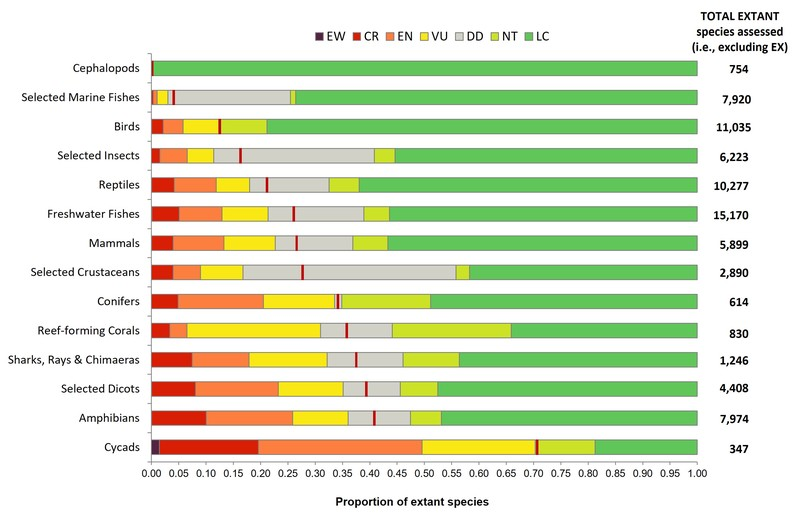
\includegraphics[width=0.9\linewidth]{figures/intro/IUCN_redlist}
    \caption{The proportion of extant (i.e., excluding Extinct) species in \citet{IUCN_redlist_2024}}
    \subcaption*{Assessed in each category for the more comprehensively assessed (i.e., at least 80\% of the group has been assessed) groups containing $\geq$ 150 species. Species are grouped into classes (with the exception of reef-forming corals, which includes species from classes Anthozoa and Hydrozoa), and are ordered according to the vertical red lines, which indicate the best estimate for proportion of extant species considered threatened (CR, EN, or VU) or Extinct in the Wild (EW). The numbers to the right of each bar represent the total number of extant species assessed for each group. \textbf{EW} - Extinct in the Wild, \textbf{CR} - Critically Endangered,\textbf{ EN} - Endangered, \textbf{VU} - Vulnerable, \textbf{NT} - Near Threatened, \textbf{DD} - Data Deficient, \textbf{LC} - Least Concern.}
    \label{fig:intro_iucn}
\end{figure}

% Drivers across types of species and ecosystem : need to highlight habitat loss, fragmentation, wildfires, overharvesting. 
This decline in Nature is undoubtly caused by direct anthropogenic drivers. According to \cite{ipbes_2022_6417333} land and sea use, reefering to the loss, fragmentation and degradation of wildlife habitat an impact of 30\%. The direct exploitation of wildlife, wild plants and trees represents 23\% of impacts. Climate change, through shifts in biogeographic conditions, impacts on species traits and genetic evolution and changes in habitat  represents 14\%, pollution represents 14\% of impacts. Finally invasive alien species represent 11\%. These drivers have differenciated impacts across ecosystems and realms \citep{ipbes_2022_6417333}. 
% Forests

For terrestrial species, land use change is the most important driver (30.5\%), driven by deforestation and agriculture, and direct exploitation follows next (21\%). 
Tropical and subtropical dry and humid forest host the greatest biological diversity. For example, they host the 10 hotspots with the greatest total number of vertebrates \citep{mittermeier_global_2011}. In such forests, habitat loss and degradation are the main drivers of reductions in species abundance and richness \citep{newbold_global_2014}. Legal and illegal selective logging destroy habitat \citep{hoare2022establishing,  bousfield_2023_large} and are combined with hunting and poaching of wildlife \citep{gallego_2020_combined}. Mediterranean forests, wooldlands and scrubs, covering 4 million km$^2$, are areas of exceptionally high diversity too \citep{Mooney2001, blondel_2010}. However, they are faced with a conjunction of threats, including climate change, land-use transformations \citep{newbold_tropical_2020} and wildfires \citep{Dupuy2019ClimateCI}. Indeed, wildfire frequency and severity are expected to increase with global warming, causing important direct and indirect costs to society including destruction of infrastructure and perturbations to economic activity \citep{wang_economic_2021}, smoke related health conditions \citep{burke_wildfire_2023, heft-neal_behavior_2023}, disrupting structural features of ecosystems \citep{Ayars2023} and threatening biological diversity \citep{Wintle2020}.
% Oceans and fish

For marine species, overexploitation is the main driver (29\%) \citep{ipbes_2022_6417333}. With 90 million tons of capture (and 141 billion \$ USD) in 2020 \citep{fao_2022_state}, fisheries stock within biologically sustainable levels have decreased to 64.6\% in 2019, from 90\% in 1974\footnote{ In this calculation, all fishery stocks are equally counted, irrespective of their abundance or catch}, driven by overfishing in the Southeast Pacific and the Mediterranean and Black seas. Assessment of fisheries stock and catch management have been proved to improve livelihoods as well as fish stocks globally \citep{melnychuk_2017_fisheries, hilborn_2020_effective}. Nonetheless, illegal, unreported and unregulated (IUU) fishing is a threat to fisheries. Estimates from 15 years ago \citep{agnew_estimating_2009} estimated it represented between 11 and 26 million tonnes of fish with a value of 10 to 23 billion \$ USD. It typically arises in weak governance contexts, with high economic incentives and barriers to enforcement \citep{iuu_2020_widjaja}. 

\section*{Concepts and challenges for a sustainable future}

% Sustainability
Anthropogenic drivers of ecosystem collapse and biodiversity decline emerge from as a consequence of the global imbalance between the rates of destruction of natural assets and their regeneration rates, driven by economic motives. Indeed, land/sea-use change, as well as overexploitation, emerge from short-term profit motives and lack of coordination from shared resources \citep{clark_profit_1973}. In this context, \textit{sustainable} practices involve considering together the dynamics and management of ecological and social system, within so-called \textit{social-ecological systems} \citep{Ostrom2009} to find trajectories that satisfy economic needs through time, while maintaining ecosystem functions, community composition and overall, biological diversity, within viable, or planetary bounds \citep{Dasgupta2007, steffen_2015_planetary}. Sustainability therefore involves considering the multiple interplays of economic forces and ecosystems, at various scales, how subsystem components may interact with each other, and how trajectories accounting for these influences can be designed. 
%, at various conceptual levels. First, it requires understanding the direct consequence of each subsystem onto the other : how do economic forces shape ecosystems? How do ecosystems shape economic forces? To answer these questions, conflicting links may be acknowledged and give rise to trade-offs

%One of the key elements is to identify the various uses and values carried by ecosystems within social-ecological systems, including conflicting perspectives\\
%From section \ref{intro:facts}, curbing the 
\textbf{More challenges, why it is interesting, big picture, to study that, in words, what are the challenges in terms of thought and why we should care, in terms of economics and big picture ideas.}


%As \textit{sustainable} practices imply a collective viewpoint, shifting away from individual decision-making, it also implies a global ecological perspective, acknowledging the interplay between social ecological system components, and the multiple functions some ecosystem underlie in social-ecological systems.
% Practices for sustainability and Aichi targets

\begin{itemize}
\item List of thematic challenges and how case studied - \textbf{link with Aichi and 30 by 30?}
\begin{itemize}
\item The first order of priority is to curb land use change for terrestrial ecosystems, to halt overexploitation and invasive species (so increase control taking space into account)
\item Also to find ways to increase habitat, while measuring the risks it poses on other aspects, in a context of climate change. 
\item Find ways to curb IUU and poaching, in difficult context where economic value is tied to the weak governance : case study of totoaba? 
\end{itemize}
\item List of big ideas that outlines the contributions : 
\begin{itemize}
\item Wildland connectivity : we need to increase the connectivity of wildlands, but also not too much; akin to managing a portfolio of resources with correlated risks?; we also want to maintain a certain level of performance for ecological criteria, and need public policy to do so.
\item Finally, as food from the sea provides X\% of global protein, aquaculture is a lever to alleviate fishing pressure and provide food and protein intake globally, as well as value for local communities. 
\end{itemize}
\end{itemize}

\section*{Bioeconomic modeling : a framework to analyze the biodiversity crisis}

As highlighted in chapter \ref{chapter1}, bioeconomic modeling has been widely used to understand the economic forces that drive resource overexploitation in terrestrial and marine settings for threatened species, the ways to address invasive species and their damages in forest landscapes, as well as ways to optimally conserve species on landscapes with varying degrees of human intervention, ranging from \textit{wilderness} to agricultural landscapes. However, this study also highlighted methodological shortcomings in bioeconomic modeling (along with \cite{Drechsler20200}) that are yet to be fully included in the  bioeconomic toolbox to help solving the biodiversity crisis. Among them, the full interplay of stochastic processes in natural and economic phenomena\footnote{While the natural resource maganagement literature has examined how risk affects decision making with risk neutral perspectives \citep{reed_1979_optimal, costello_optimal_2008}, risk and tipping \citep{costello_renewable_2019} and risk averse perspectives \citep{McGoughPlantingaCostello+2009,kapaun_does_2013,TAHVONEN2018659}, the full effect of different attitudes towards risk and consumption smoothing is a recent endeavor. Disentangling the effect of risk and time preferences, \citep{quaas_2019_insurance, AugeraudVeron2019} characterize the insurance value of capital. Recently, \citep{KELSALL2023102855} characterize the effect of preferences towards risk and intetemporal variability of income on resource extraction.}, the inclusion of participatory approaches, 
% List the shortcomings from the literature : not so sure about that. 

\clearpage
First, the full extent of natural and economic stochasticity still remains to be studied as it is a burning issue in the context of climate change and increased environmental stochasticity.
   Among other 
  
  on resource extraction has only recently been studied (Kelsall). The relative effect of risk aversion and intertemporal income variability has been to showcase the insurance role of biological diversity, but has yet to be fully analyzed   disentangling the role of different sources of risk, temporal consumption smoothing and intertemporal variability has highlighted insurance values of biodiversity, but only recently been studied  (see 


Among these dimensions, I chose to focus on the roles of habitat connectivity and market structure, as they are key to understand and adress the two most important drivers of global biodiversity decline, land/sea use change and overexploitation of resources. 

two components are key to adressing major drivers of biodiversity decline



% Reprendre cela : 
Stochasticity governs ecological and economic processes, and has gradually been included in decision-making from resource managers, and how risks affect resource extraction (Reed, Costello, Costello et al), role of multiple risks together is being studied (Costello et al), and how dynamic choices, uncertainties etc are being considered (check intro by Claudia). 
% 
\clearpage


What should I say in the general introduction of my thesis? 

\begin{itemize}
\item Une page qui résume : le déclin de la biodiversité, l'économie bioéconomique, la contribution méthodologique de la thèse, et les résultats nouveaux. 

\item Introduction générérale thématique : le déclin de la biodiversité / 3-5 pages avec des graphiques. 
\begin{itemize}
\item Le déclin de la biodiversité de façon générale
\item Par ecosystème et taxon : on parlera alors de poissons, d'espèces invasives, de forêts
\item En rajoutant un petit quelquechose sur le changement climatique
\item Les causes sont à chercher du coté des hommes
\end{itemize}

\item D'où la necessité d'une approche par les sciences sociales, et l'économie peut y apporter beaucoup, elle l'a déja fait : social ecological systems, JEEM. 
\item Pourquoi l'économie et la modélisation bioéconomique?
\begin{itemize}
\item Un problème d'externalité global, de biens publics, de valeurs d'options, d'informations e.g. tous les problèmes spécifiques à l'économie de l'environnement
\item Un outil permettant la modélisation et la prospective: c'est à dire la description, sur base axiomatique, des comportements, à la fois individuels, non coopératifs, et de politique publique. 
\item Qui permet d'articuler grâce à un langage partagé différent champs de connaissance, notamment de dialoguer avec les sciences du vivant
\item Nonobstant les contributions
\item Il existe des champs d'application inexplorés, ou des questions importantes non résolues : bien lister ici les dimensions : marché, espace, politique publique/gestion privée. \\
From the review:
\begin{itemize}
\item Stochasticity : how stochasticity governs ecological and economic processes is a recent strand, but studied (costello, augereau véron, quaas and Baumgartner). Remain an open question as to how do people respond to uncertain and risky contexts, with the limited possibility of insurance; mentionner des choses à la Romain, genre risques reliés : stochasticité de la ressource écologique et incertitude autour de la détection des invasive species etc. 
\item Community perspective for ecosystem based conservation planning, e.g. interaction between several species at the landscape level
\item The role of spatial processes, for movement, different habitat quality, understanding how space changes results in combination with other determinants of bioeconomic models (Sanchirico, Costello as well)
\item Intricate property rights, ranging from the most localy complex in terms of types of interactions (externality locally), local competition for resource, different levels of political management, but also different types of market structure

\item Incorporating different value types, including indigenous knowledge, in bioeconomic modeling for policy making

\item incorporating more evidence from quasi experimental methods in the results
\end{itemize}
\end{itemize}

\item \textbf{ On a donc deux éléments bien identifiés dans la recherche et les questions qu'ils posent }: l'espace et la structure de marché. 
\item La structure de marché : 
\begin{itemize}
\item Question bien vieille dans la litérature sur les ressources naturelles: Solow, Hotelling etc
\item Moins bien tranchée sur la question des ressources renouvelables : rhinos (AER), foresterie etc ... 
\item On l'étudie donc dans un cas précis, c'est le chapitre 2
\end{itemize}
\item La question de l'espace : 
\begin{itemize}
\item L'espace est une dimension importante à prendre en compte, car il conditionne l'exploitation des ressources, autant que comment les décisions doivent être prises : ce qui change (Sanchirico et Costello)
\item C'est un challenge qui pose des questions de politique publique : la gestion de l'espace, dans un contexte de fragmentation, de prévention des risques etc est cruciale 
\item Il faut aussi comprendre comment l'espace, et les processus écologiques qu'il construit, sont formés par les individus [à raffiner] c'est le chapitre 3
\end{itemize}
\item Bien mentionner que l'intégralité des données, codes etc sont disponibles gratuitement et librement. 
\end{itemize}

\textbf{What's left to do}
\begin{itemize}
\item List contributions from the literature review, and find a way to put more into it. 
\item Find references and graphs from the institutions to document biodiversity loss
-> IPBES?
\end{itemize}
\clearpage

\section{New intro}
\subsection{Plan global}
Idée d'organisation : 
\begin{enumerate}
\item Documenter la crise de la biodiversité : état et causes\\
Un point de plus sur l'habitat, les poissons, et les usages des forêts
\item La nécessité d'une trajectoire soutenable : définition de la soutenabilité, actions à engager, afin d'avoir un usage soutenable de la nature
\item Un cadre d'analyse pour les penser
\item Les limites existantes
\item Comment les surmonter, et appliquer cela aux cas qui m'intéressent?
\end{enumerate}
\subsection{Plan détaillé}

 
 



\begin{enumerate}
\item Lay the facts : global biological diversity decline (1-2 pages)
\begin{itemize}

\item An overall decline over time : 
\begin{itemize}
\item Across taxa : for types of animals, document extinctions across taxa and decline in populations
\item Across ecosystems : terrestrial and marine, forests etc
\end{itemize}

\item What is biological diversity? How can we define it? What values does it call for? \textit{Est ce que ça a vraiment sa place ici?} - peut être plutôt note de bas de page, sur les difficultés du concept etc, mais on se dit richness and abundance across the world

\item The causes are man made, on land and at sea : land use change, overexploitation, habitat destruction and fragmentation, as well as climate change (for wildfire)
\\
Notion of direct and indirect drivers\\

Rajouter une bonne couche sur la nécessité de (i) pas trop exploiter et pourquoi; et (ii) sur la fragmentation de l'habitat (avec pas mal de concepts écologiques, genre surface, fragmentation, stepping stones etc)
\item Weak substitutability of biological diversity.\\
\item International and global policy goals in IPBES, Biodiversity Strategy for 2050 etc, pour ancrer les objectifs de la thèse.
\end{itemize}

\item Lik with substitutability, and need for sustainable approaches : can use the table SPM1

\item Need a unifying method, conceptual body, to remedy this crisis : find pathways towards a sustainable future etc\\
$\Rightarrow$ Bioeconomic modeling : what it is

\begin{itemize}
\item What it does : mix together ecological dynamics and economic drivers
\item Strengths : process based, out of sample, policy design
\item Applied to various ecosystems : forestland a lot, oceans and fisheries, and agricultural land to have several \\
Maybe list some results?
\end{itemize}

\item The current state of biodiversity calls for an ``ecosystem centered'' management\\
\textit{Unconfortable with that, but it allows to introduce bioecon modeling, and highlight the shortcomings based on empirical facts}
\begin{itemize}
\item Ecosystems feature different uses, different species, offer different risk and benefits etc : cases of forests (risks of wildfire, habitat to biodiversity, forestry industry, leasure); and oceans (fisheries, conservation of habitat, leasure).
\item The literature has gradually evolved towards encompassing the many dimensions of ecosystem based management, but shortcomings remain : 
\begin{itemize}
\item Stochasticity : how stochasticity governs ecological and economic processes is a recent strand, but studied (costello, augereau véron, quaas and Baumgartner). Remain an open question as to how do people respond to uncertain and risky contexts, with the limited possibility of insurance; mentionner des choses à la Romain, genre risques reliés : stochasticité de la ressource écologique et incertitude autour de la détection des invasive species etc. 
\item Community perspective for ecosystem based conservation planning, e.g. interaction between several species at the landscape level
\item The role of spatial processes, for movement, different habitat quality, understanding how space changes results in combination with other determinants of bioeconomic models (Sanchirico, Costello as well)
\item Intricate property rights, ranging from the most localy complex in terms of types of interactions (externality locally), local competition for resource, different levels of political management, but also different types of market structure

\item Incorporating different value types, including indigenous knowledge, in bioeconomic modeling for policy making
IPLCs have been using fire to promote herbaceous vegetation
and useful game or plant species (Pechony \& Shindell,
2010; Valladares et al., 2014). Such historical practices and
other land-use legacies combined with more recent driving
forces, such as land abandonment and fire suppression
strategies, have been playing a major role in reshaping the
Mediterranean landscapes (Blondel, 2006; Gauquelin et al.,
2018; Marlon et al., 2008; Valladares et al., 2014).

\item incorporating more evidence from quasi experimental methods in the results
\end{itemize}
\end{itemize}
\item In this dissertation, I chose to focus on space and market structure across 2 different types of ecosystems
\begin{itemize}
\item Space \& Market structure : make up policy, conceptual and methodological challenges, as they adress the principal causes of global biodiversity decline and foster technical and methodological challenges, as highlighted by our review and other. 
\item Space on terrestrial landscapes is important to tackle main causes of species decline: 

\begin{itemize}
\item Classical arguments : featuring space in traditional models allows to understand better aggregate behavior (Sanchirico); externalities arise from spatial dependence, and optimal behavior can be characterized in some cases (Costello)

\item Spatial dependence creates problems, but landscape \textbf{connectivity} is of the essence : 
\begin{itemize}
\item Hu et al
\item Tischendorf \& Farig
\item May et al
\item Fahrig
\item Hanski
\item Fischer \& Lindenmayer
\end{itemize}

\item Forests support a variety of functions and risks, benefits and costs; these risks and benefits have distinct spatial patterns, and occur at a large scale, calling for an aggregate scale approach; different phenomena are characterized by different scales, different time frames and different ??? but connectivity is an important feature that structures ecological processes; raises specific challenges with spatial optimization; spatial management of connectivity with multiple use/functions ecosystems is complicated, but useful in terms of policy and methods\\
Additionally, in a context of resource scarcity, space can be a driver of policy success for both resource preservation and wildfire prevention. 
\item Spatial heterogeneity drives movement; spatial ressources are difficult to manage as they create spatial externalities, that are dynamic through time; it has long been considered that movement is an exogenous process, or driven exclusively by ecological features; besides fragmentation, as well as corridors etc, human actions at a more local scale can change the pattern of spatial movement, especially in the case of invasive species. Petite envolée sur le fait que la géographie est le résultat d'un processus social? When possible, people may fence, to resolve the externality; in doing so, they may have a better use of the resource (e.g. halt overexploitation) but undermine landscape connectivity (e.g. increase fragmentation); it is shown that not all fences are bad, and connectivity is good if heterogeneity exists; 

\item Leverages specific challenges when dealing with dynamics : dimensionality curse, which gives rise to several types of methods to solve the problem, when complexity dimensions can be trimmed (chapter on connectivity uses a simplified dynamic with a lot of space and state dependence, while fences uses a lot of space, non simplified dynamics, but with no state dependence)
\end{itemize}

\item Market structure matters for resource exploitation

\begin{itemize}
\item In the harvesting literature, it is often considered that marginal revenue is constant as prices are determined by an international market. Additionally, open access is a key feature of the commons, and a small group of people seldom controls a complete market.
\item However, some specific cases of endemic resources, such as wildlife trade, in informal contexts, can be characterized by restricted access
\item A monopolist may be a conservationist's best friend : intuitively, restrict quantities to maximize profits. This is dependent on market specifics, discounting etc (Hanesson)
\item Additionally, competition in intricate settings can trigger weird dynamic, according to existing papers 
\end{itemize} 
\end{itemize}
\item That's how I choose to adress them 
\begin{itemize}
\item Summary of research work
\end{itemize}
\textit{Or should that be integrated with the previous point? }
\end{enumerate}

\clearpage

\section*{Summary of publications and conferences}
\singlespacing
\textbf{Chapter 1 :  Bioeconomic Models for Terrestrial Social Ecological System Management : a Review}, S.Jean and L. Mouysset\\
\href{https://github.com/sim-jean/review-irere}{Replication code} and \href{https://zenodo.org/records/6656433}{data} are freely accesible
\begin{itemize}
\item Published in \textit{International Review of Environmental and Resource Economics}\\
 DOI : 10.1561/101.00000131
\item Presentations : 
\begin{itemize}
\item European Association of Environmental and Resource Economists (EAERE) Annual Conference, Rimini, 2022
\item ABIES Doctoral Days - Best Poster Award, 2022
\end{itemize}
\end{itemize}
%
\textbf{Chapter 2 : The Wildfire-Habitat Connectivity Dilemma: a Graph Theoretical Approach to Landscape Management}, S.Jean and L. Mouysset\\
\href{https://github.com/sim-jean/Landscape_connectivity_dilemma}{Replication code and data} are freely accessible
%
\begin{itemize}
\item Working paper
\item Presentations : 
\begin{itemize}
\item BINGO Seminar, CIRED, 2023
\item Interdisciplinary PhD in Sustainable Development, Columbia University, 2023
\end{itemize}
\end{itemize}
%
\textbf{Chapter 3 : Fences - the Economics of Movement in Mobile Public Bads}\\
\href{https://github.com/sim-jean/fences}{Replication code and data} are freely accessible
%
\begin{itemize}
\item Working paper
\item Presentations : 
\begin{itemize}
\item French Association of Environmental and Resource Economists, Université Savoie Mont-Blanc, 2024
\item Parisian PhD Seminar in Environmental Economics, Nogent sur Marne, 2024
\item CIRED Internal Seminar, 2024
\end{itemize}
\end{itemize}
%
\textbf{Chapter 4: Little downside and susbtantial gains result from farming of \textit{Totoaba Macdonaldi}}, J. Lawson, S.Jean (co-first authors), A. Steinkruger, M. Castellanos-Rico, G.M. Goto, M.A. Cisneros-Mata, E. Aceves Bueno, M.M. Warham, A.M. Sachs and S.D. Gaines\\
\href{https://github.com/julawson/conservation_farming_totoaba}{Replication code and data} are freely accessible.
%
\begin{itemize}
\item Under review at \textit{NPJ Ocean Sustainability}
\item Presentations:
\begin{itemize}
\item BIOECON Network Annual Conference, University of Santiago de Compostela, 2023
\item Trade and the Environment, Paris Saclay Applied Economics, 2023
\item European Association of Environmental and Resource Economists Annual Conference, University of Leuven, 2024
\end{itemize}
\end{itemize}
%

